\chapter{Euler Graphs and Hamilton Graphs}

\begin{descr}
    TODO
\end{descr}

\section{Euler Graphs}\index{Euler Graphs}
\subsection{Euler 1736: K�nigsberger Br�ckenproblem}
Is it possible to do a round walk crossing every bridge exactly once?\\
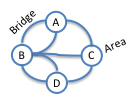
\includegraphics{diagrams/koenigsberg.png}

\begin{example}
    
\includegraphics{diagrams/haus_vom_nikolaus.png}    
\end{example}

\begin{definition}
Let $G$ be a finite undirected graph. A path $e_{1}..e_{t}$ is called a \deftxt{euler path}
if every edge in $E$ occurs exactly once in the list.\\
A graph is a \deftxt{euler graph} if it has a euler path.
\end{definition}

\begin{theorem}
    A finite connected graph is a euler graph if and only if:
    \begin{enumerate}
        \item It ha eiter exactly two nodes of odd degree.
        or
        \item All nodes have even degree.
    \end{enumerate}
\end{theorem}

In the last case the path is a cycle. In the first case no euler path is a cycle.
Check is possible in linear time.

\begin{prooof}
    $">"$ Let $G=(V,E)$ be a graph that has a euler path that is not a cycle. Let $\mid E \mid=k$
    $\circ  \xrightarrow{e_{1}} \circ \xrightarrow{e_{2}} ... \circ \xrightarrow{e_{k}}$
    In this path $v_{1}$ and $v_{k+1}$ have od degreee and all other nodes have even degree. 
    Now consider the case teht $G$ has a euler cycle.\\
    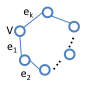
\includegraphics{diagrams/proof21.png} \\
    Hence every node has even degree. \\[2mm]
    
    $"<"$ Let $G$ be a graph with exactly two nodes with odd degree, let this be $a$ and $b$.
    We contradict a euler path as follows:\\
    Start at node $a$ and folow an edge ?inktt? on a. $a -- v$
    If the node that we currently deal with is neither $a$ nor $b$ then passing this node will use up
    two edges. If we look at the residual degree at $v$, it is an even number. If at some point we reach a node which 
    we can enter but not leave it must be $b$.
\end{prooof}
